
\subsection{Heuristics}~\label{subsec:heuristics}

\autoref{fig:global-heuristics} shows the performance of \tool with different
heuristics turned on and off. First we consider turning three optimizations off.
\autoref{fig:globaldontfilter} compares against when we turn off filtering short
and non-trivial \pr clauses. \autoref{fig:global-max-length} compares against
when we filter only clauses of length $10$ or greater.
\autoref{fig:global-no-shrink} compares to when we decide not to shrink clauses.
When we disable all three optimizations, the performance is significantly,
especially on \texttt{perfect-matching}, \texttt{mutilated-chessboard}, and
\texttt{register-allocation} benchmarks.

Additionally, we consider potential improvements to the heuristics used in
\tool. Three possible options are to change the time limit of preprocessing, try
to efficiently sort the first propagated variable $i$ and try to sort the second
propagated variable $j$. \autoref{fig:global-time-limit} does the first, by
setting the pre-processing time limit to 100 seconds.
\autoref{fig:global-time-limit}. \autoref{fig:global-sort-i} does the second by
propagating $i$ in order of which literals occurs most frequently in the
original formula. Finally, \autoref{sub@fig:global-touched} does the the third,
for each $i$ propagated, for each other $j$, it counts the number of clauses
that contain $j$ and $i$ (or a literal propagate by $i$). It then picks $j$
based on which has the highest of this score.


\begin{figure*}[!t]
    \centering
    \begin{subfigure}[t]{0.3\textwidth}
        \centering
        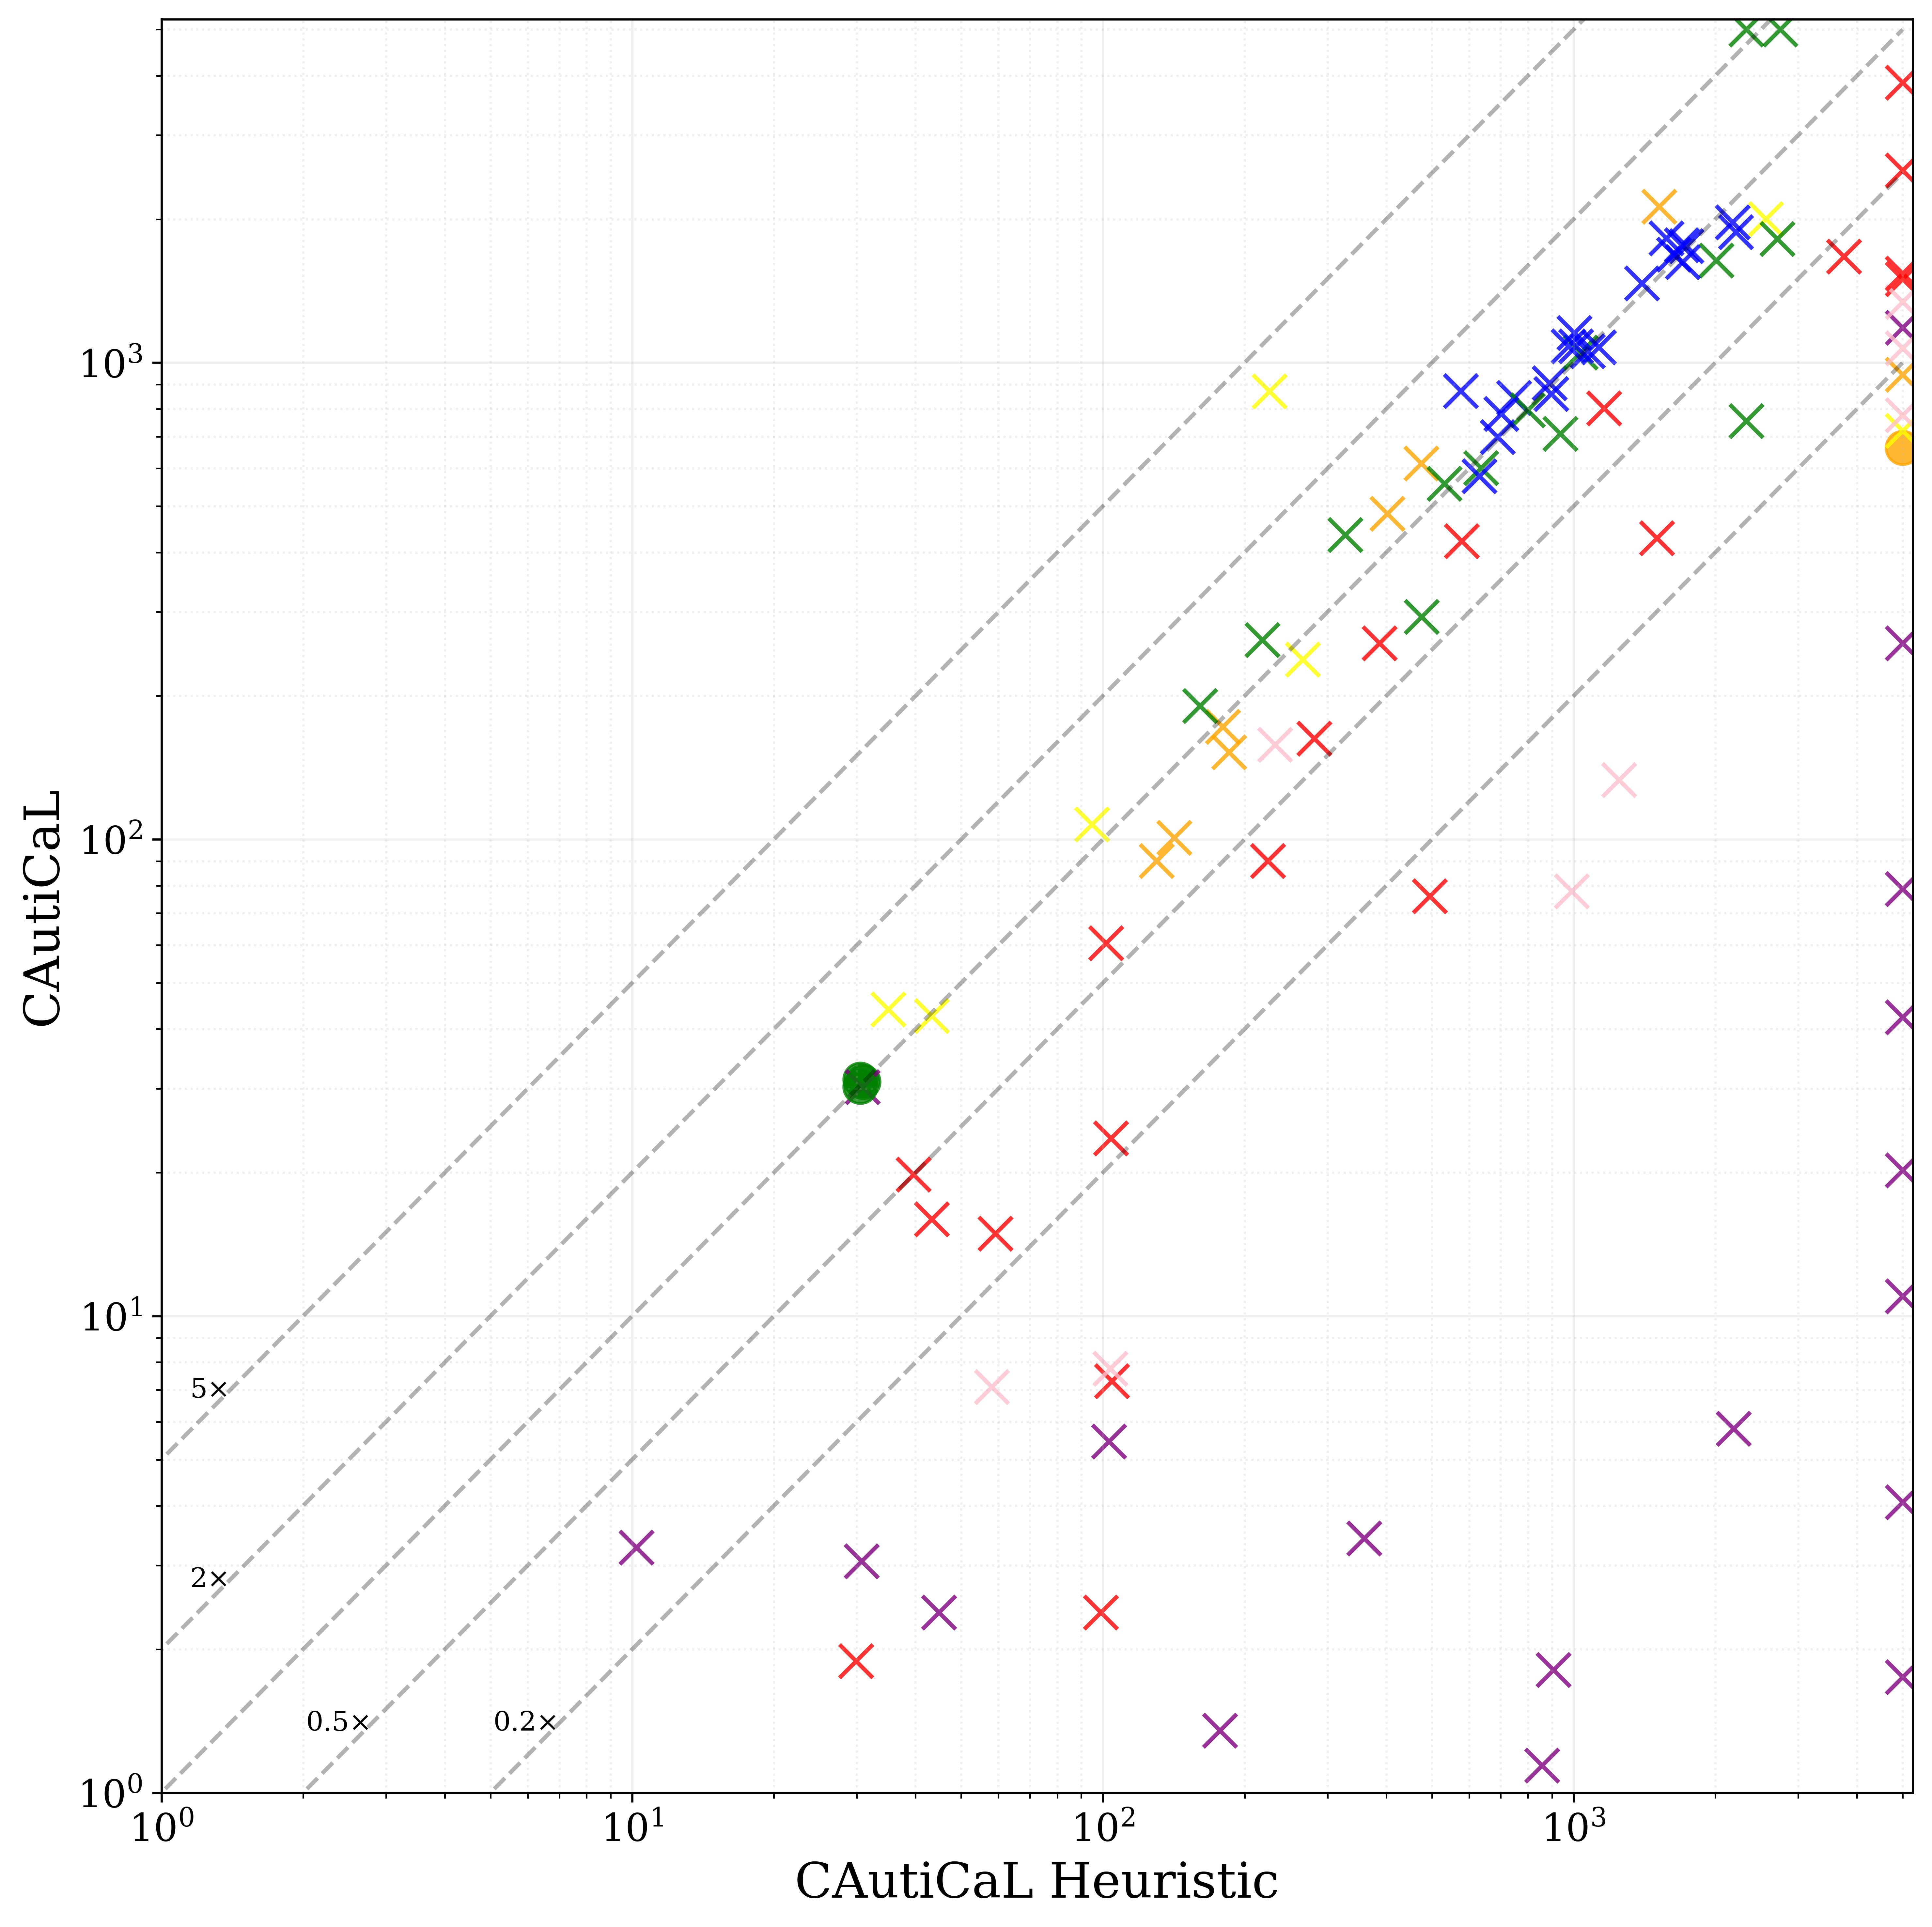
\includegraphics[width=\textwidth]{figs/globaldontfilter_heuristic_comparison.jpg}
        \caption{No filter}
        \label{fig:globaldontfilter}
    \end{subfigure}
    \begin{subfigure}[t]{0.3\textwidth}
        \centering
        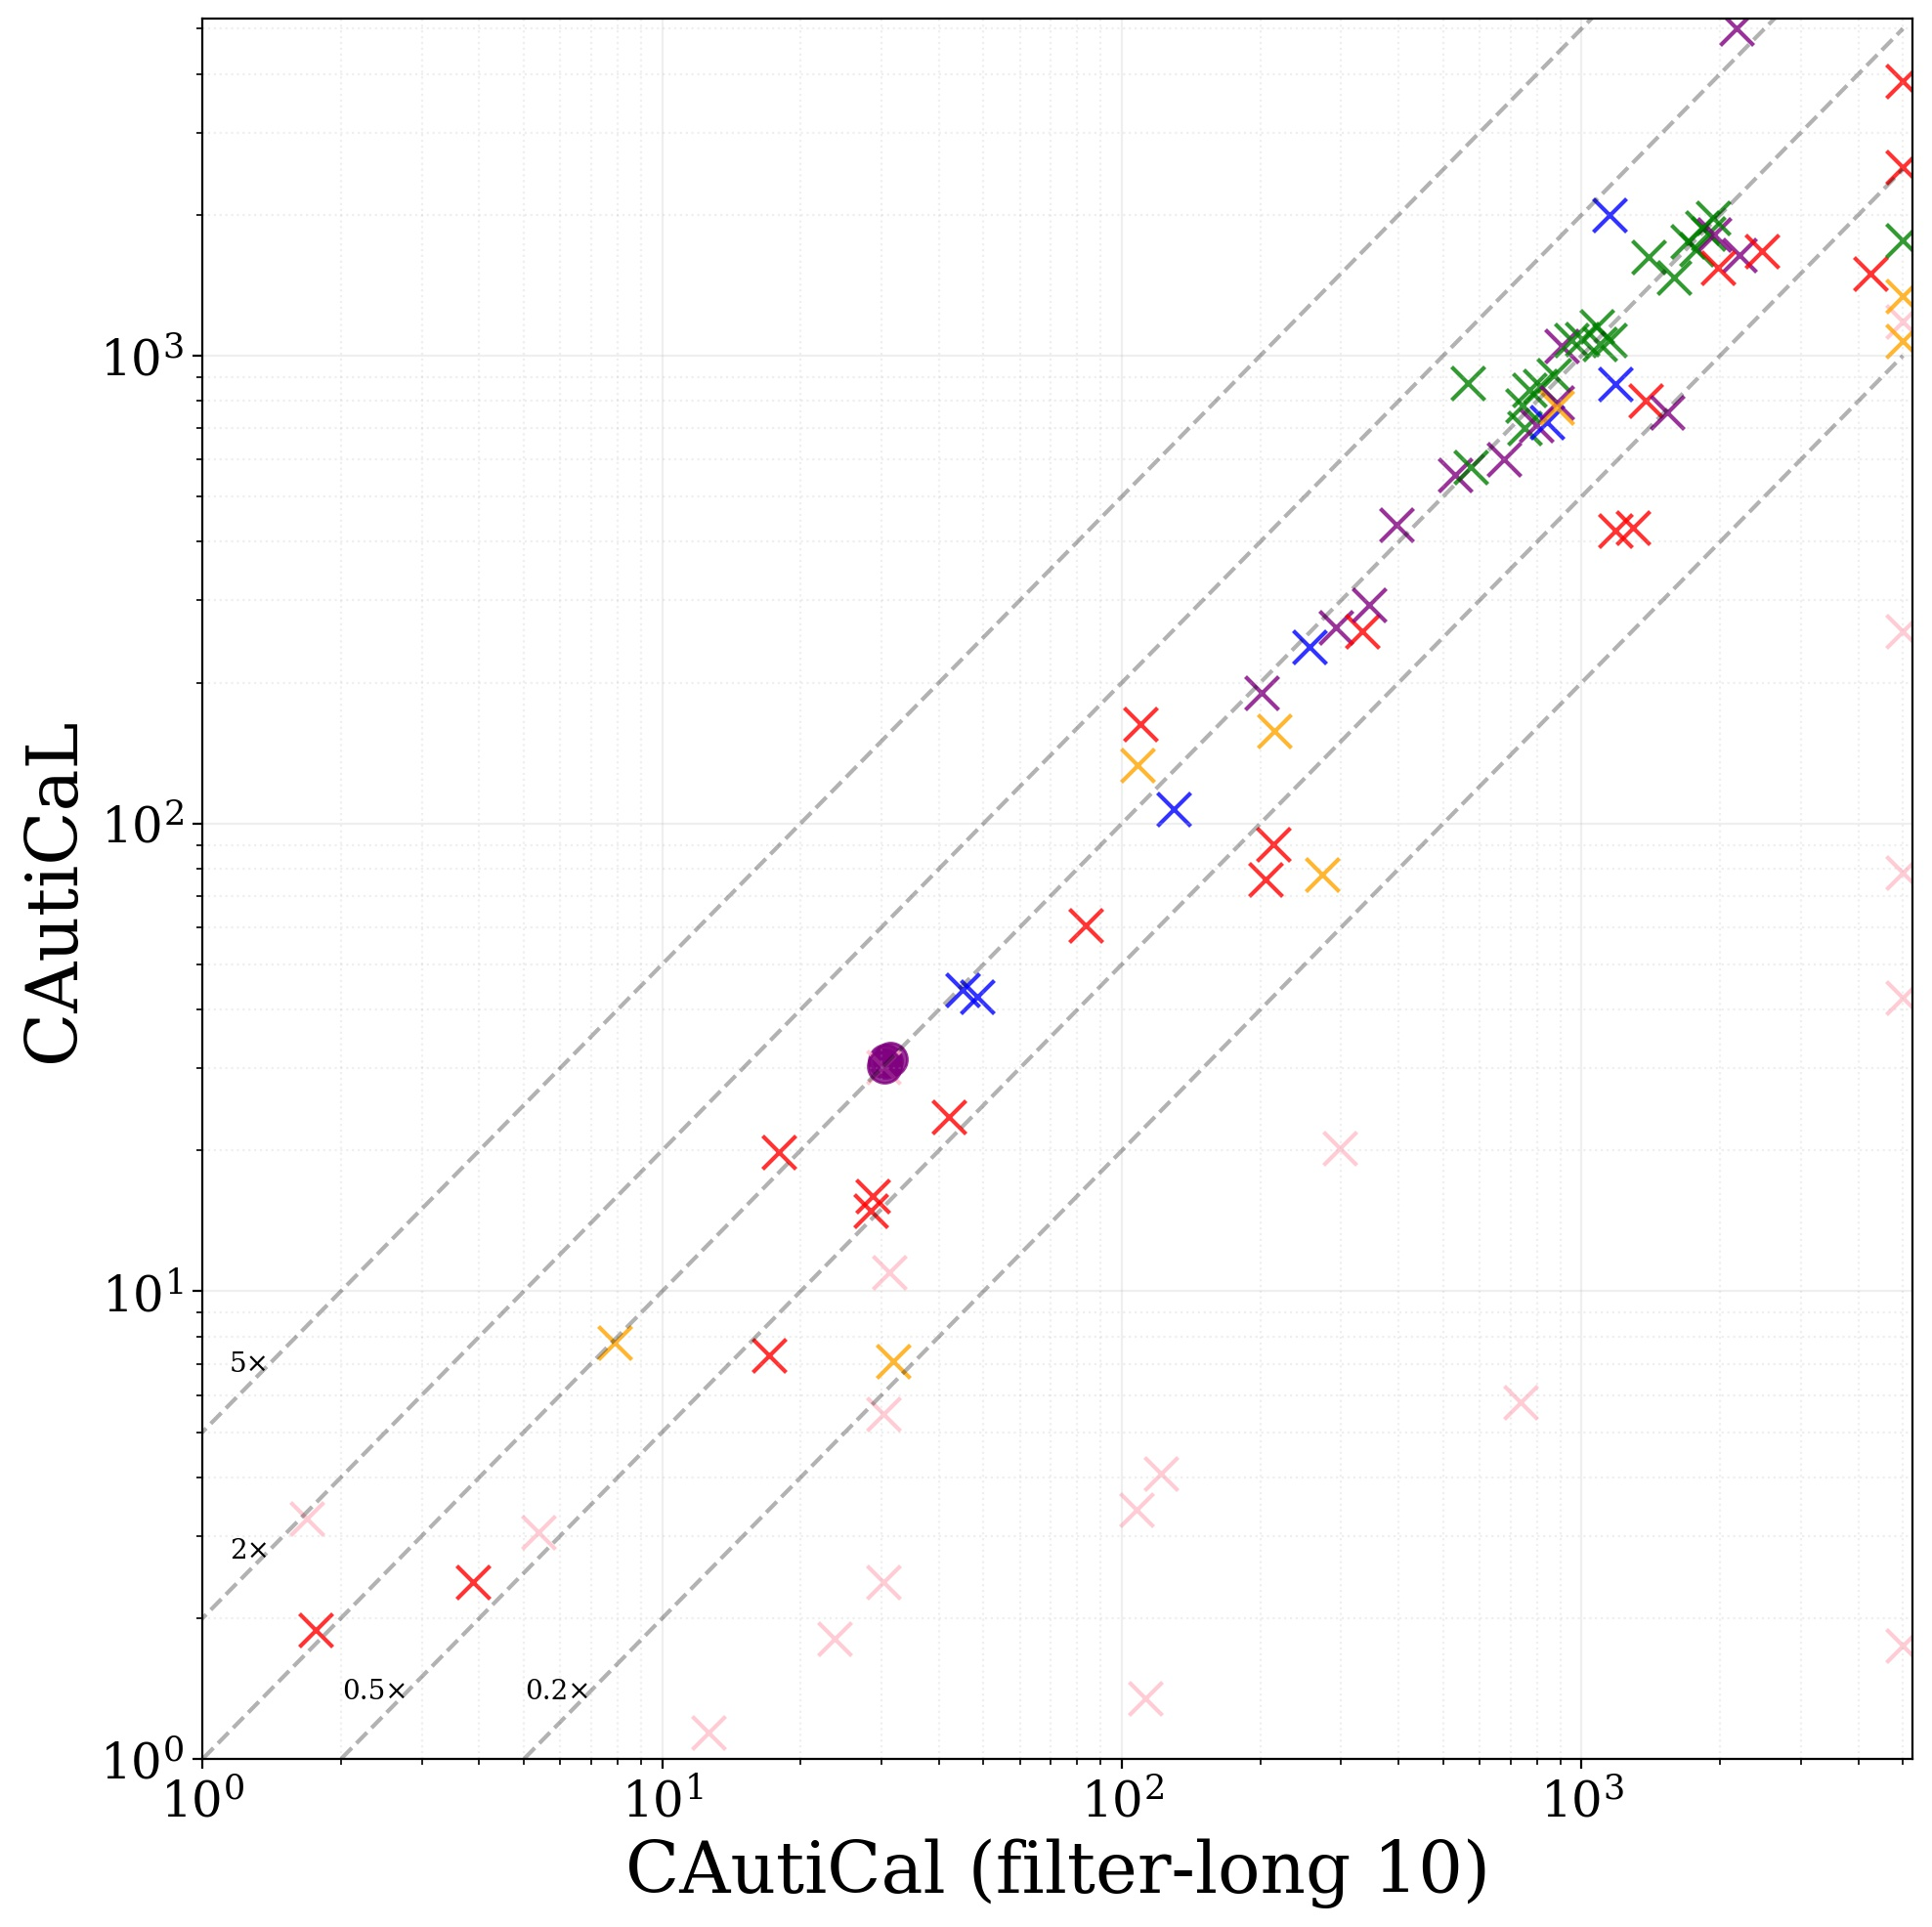
\includegraphics[width=\textwidth]{figs/globalmaxlen_heuristic_comparison.jpg}
        \caption{Max length}
        \label{fig:global-max-length}
    \end{subfigure}
    \begin{subfigure}[t]{0.3\textwidth}
            \centering
            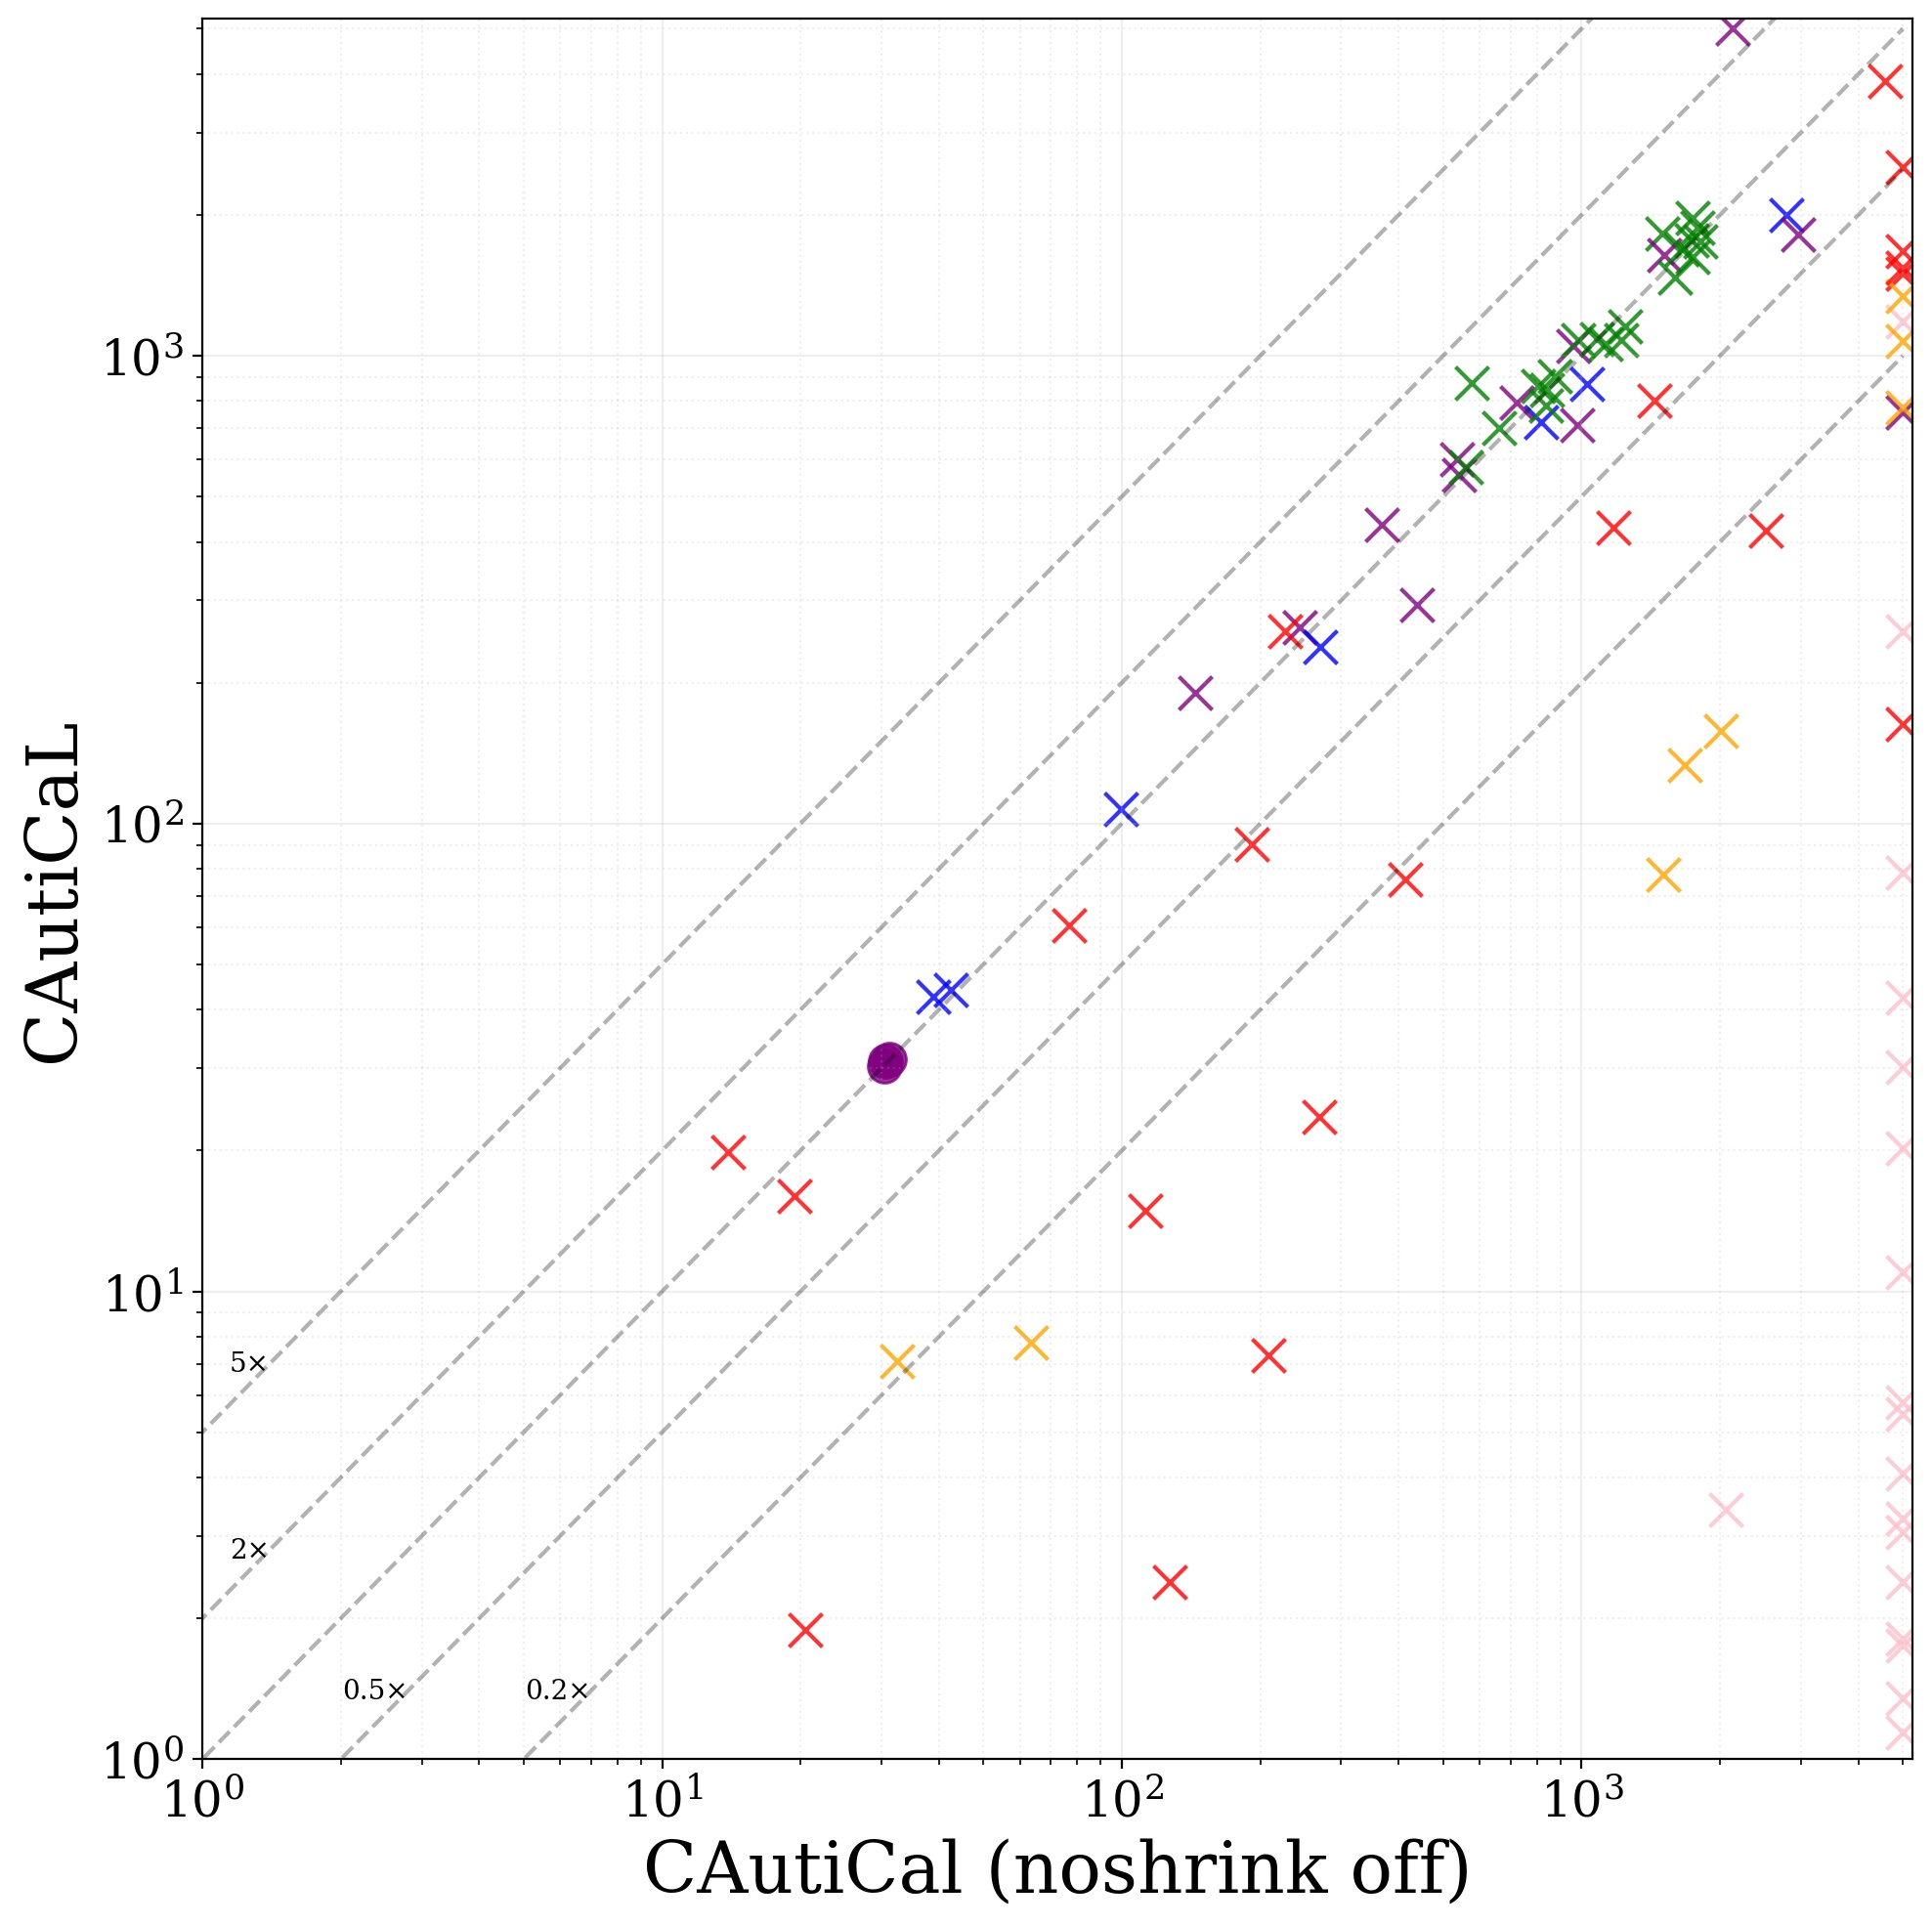
\includegraphics[width=\textwidth]{figs/globalnoshrink_heuristic_comparison.jpg}
            \caption{No shrink}
            \label{fig:global-no-shrink}
    \end{subfigure}
    \begin{subfigure}[t]{0.3\textwidth}
        \centering
        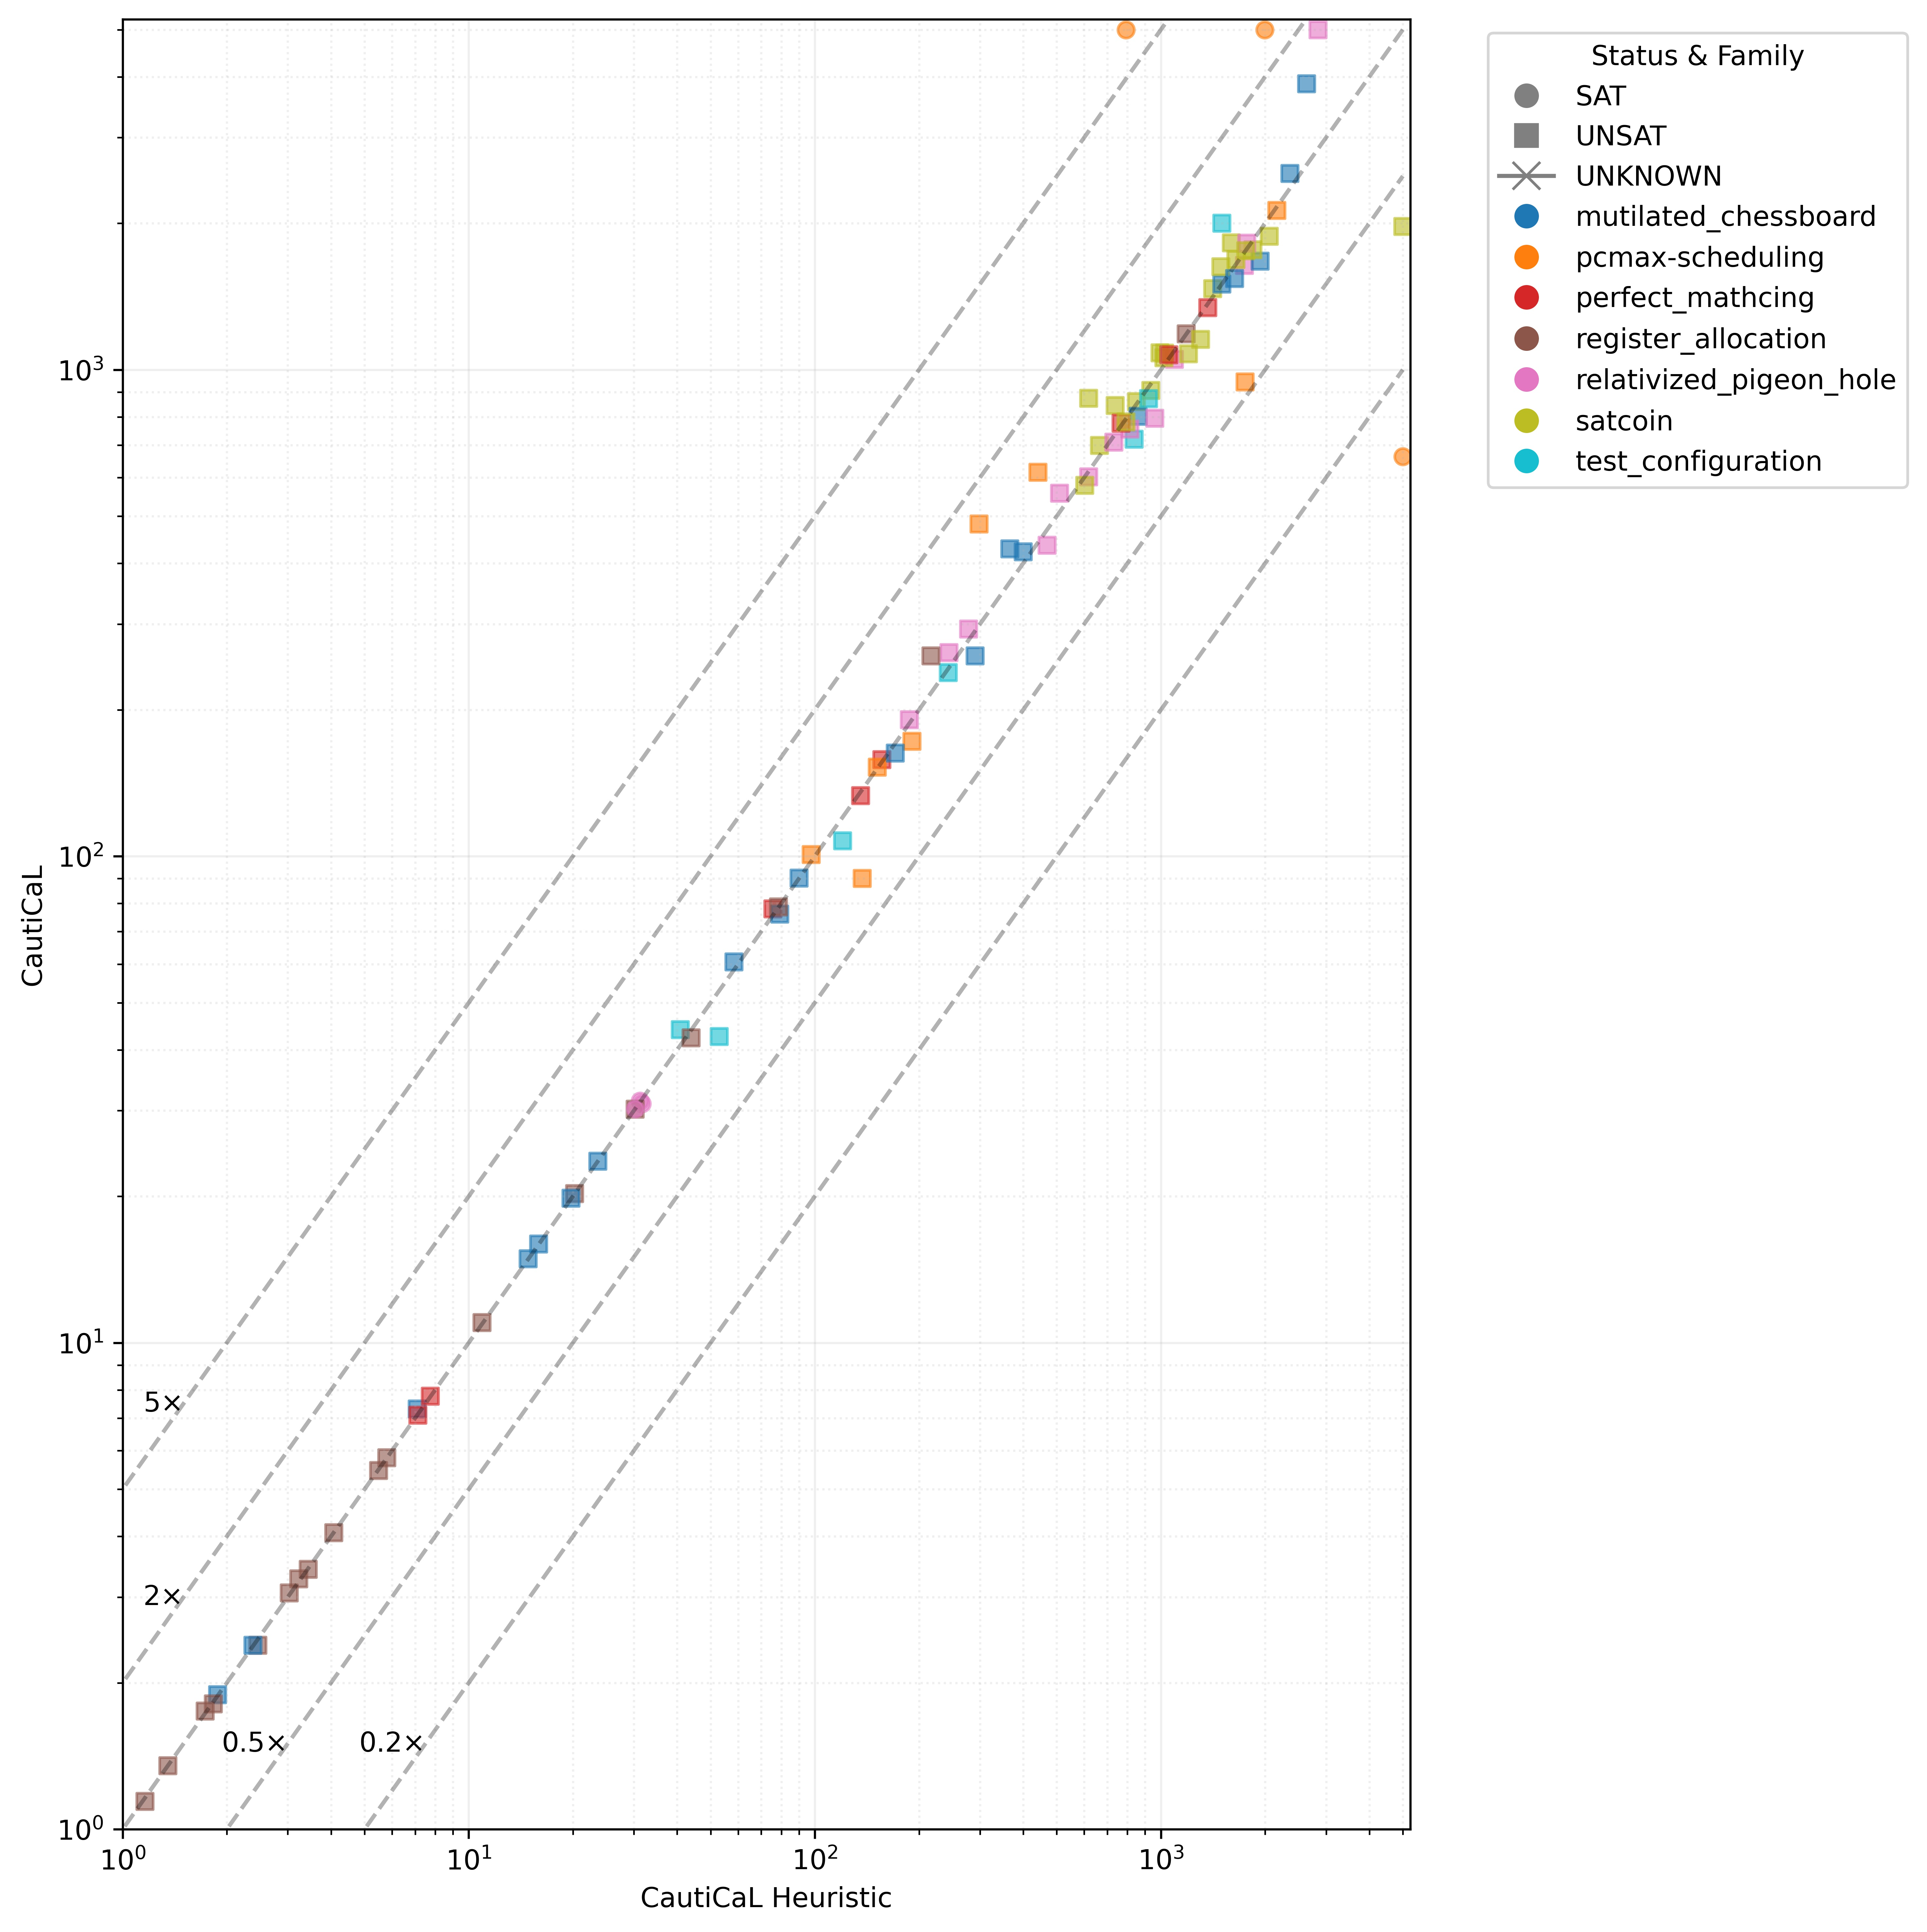
\includegraphics[width=\textwidth]{figs/global_time_lim_heuristic_comparison.jpg}
        \caption{Time limit}
        \label{fig:global-time-limit}
    \end{subfigure}
    \begin{subfigure}[t]{0.3\textwidth}
        \centering
        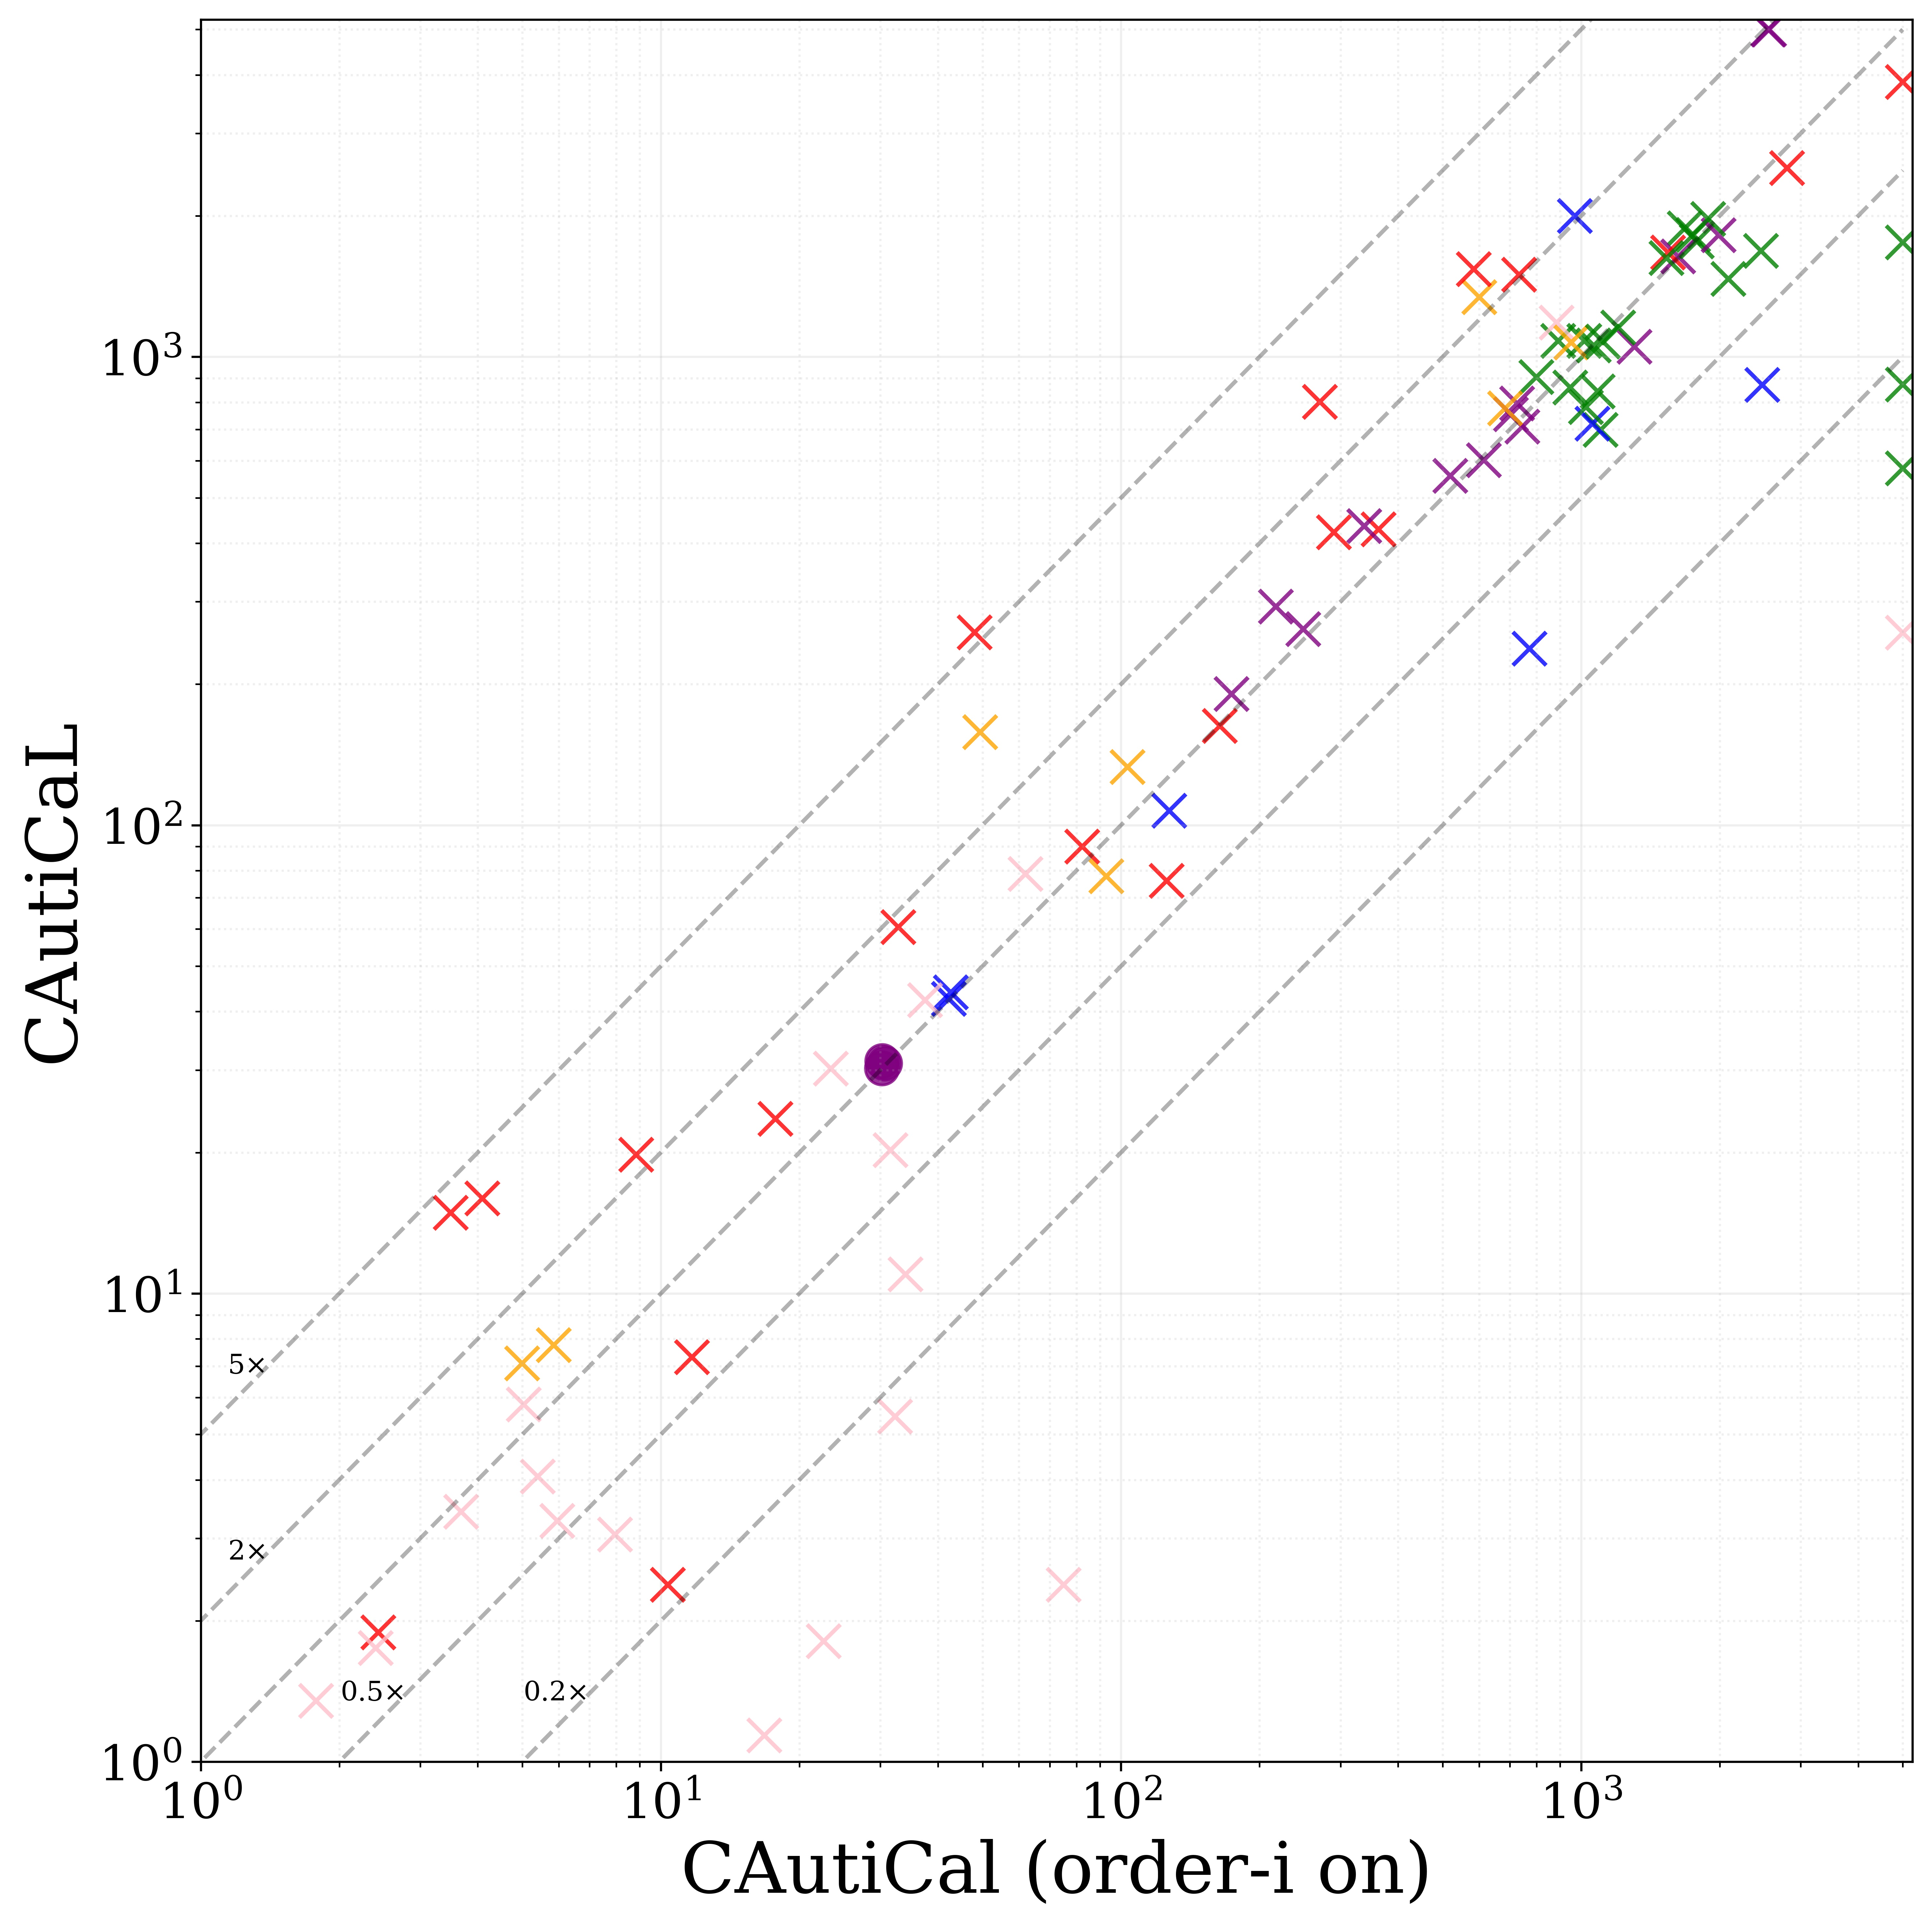
\includegraphics[width=\textwidth]{figs/globalisort_heuristic_comparison.jpg}
        \caption{Sort $i$ beforehand by frequency used}
        \label{fig:global-sort-i}
    \end{subfigure}
    \begin{subfigure}[t]{0.3\textwidth}
        \centering
        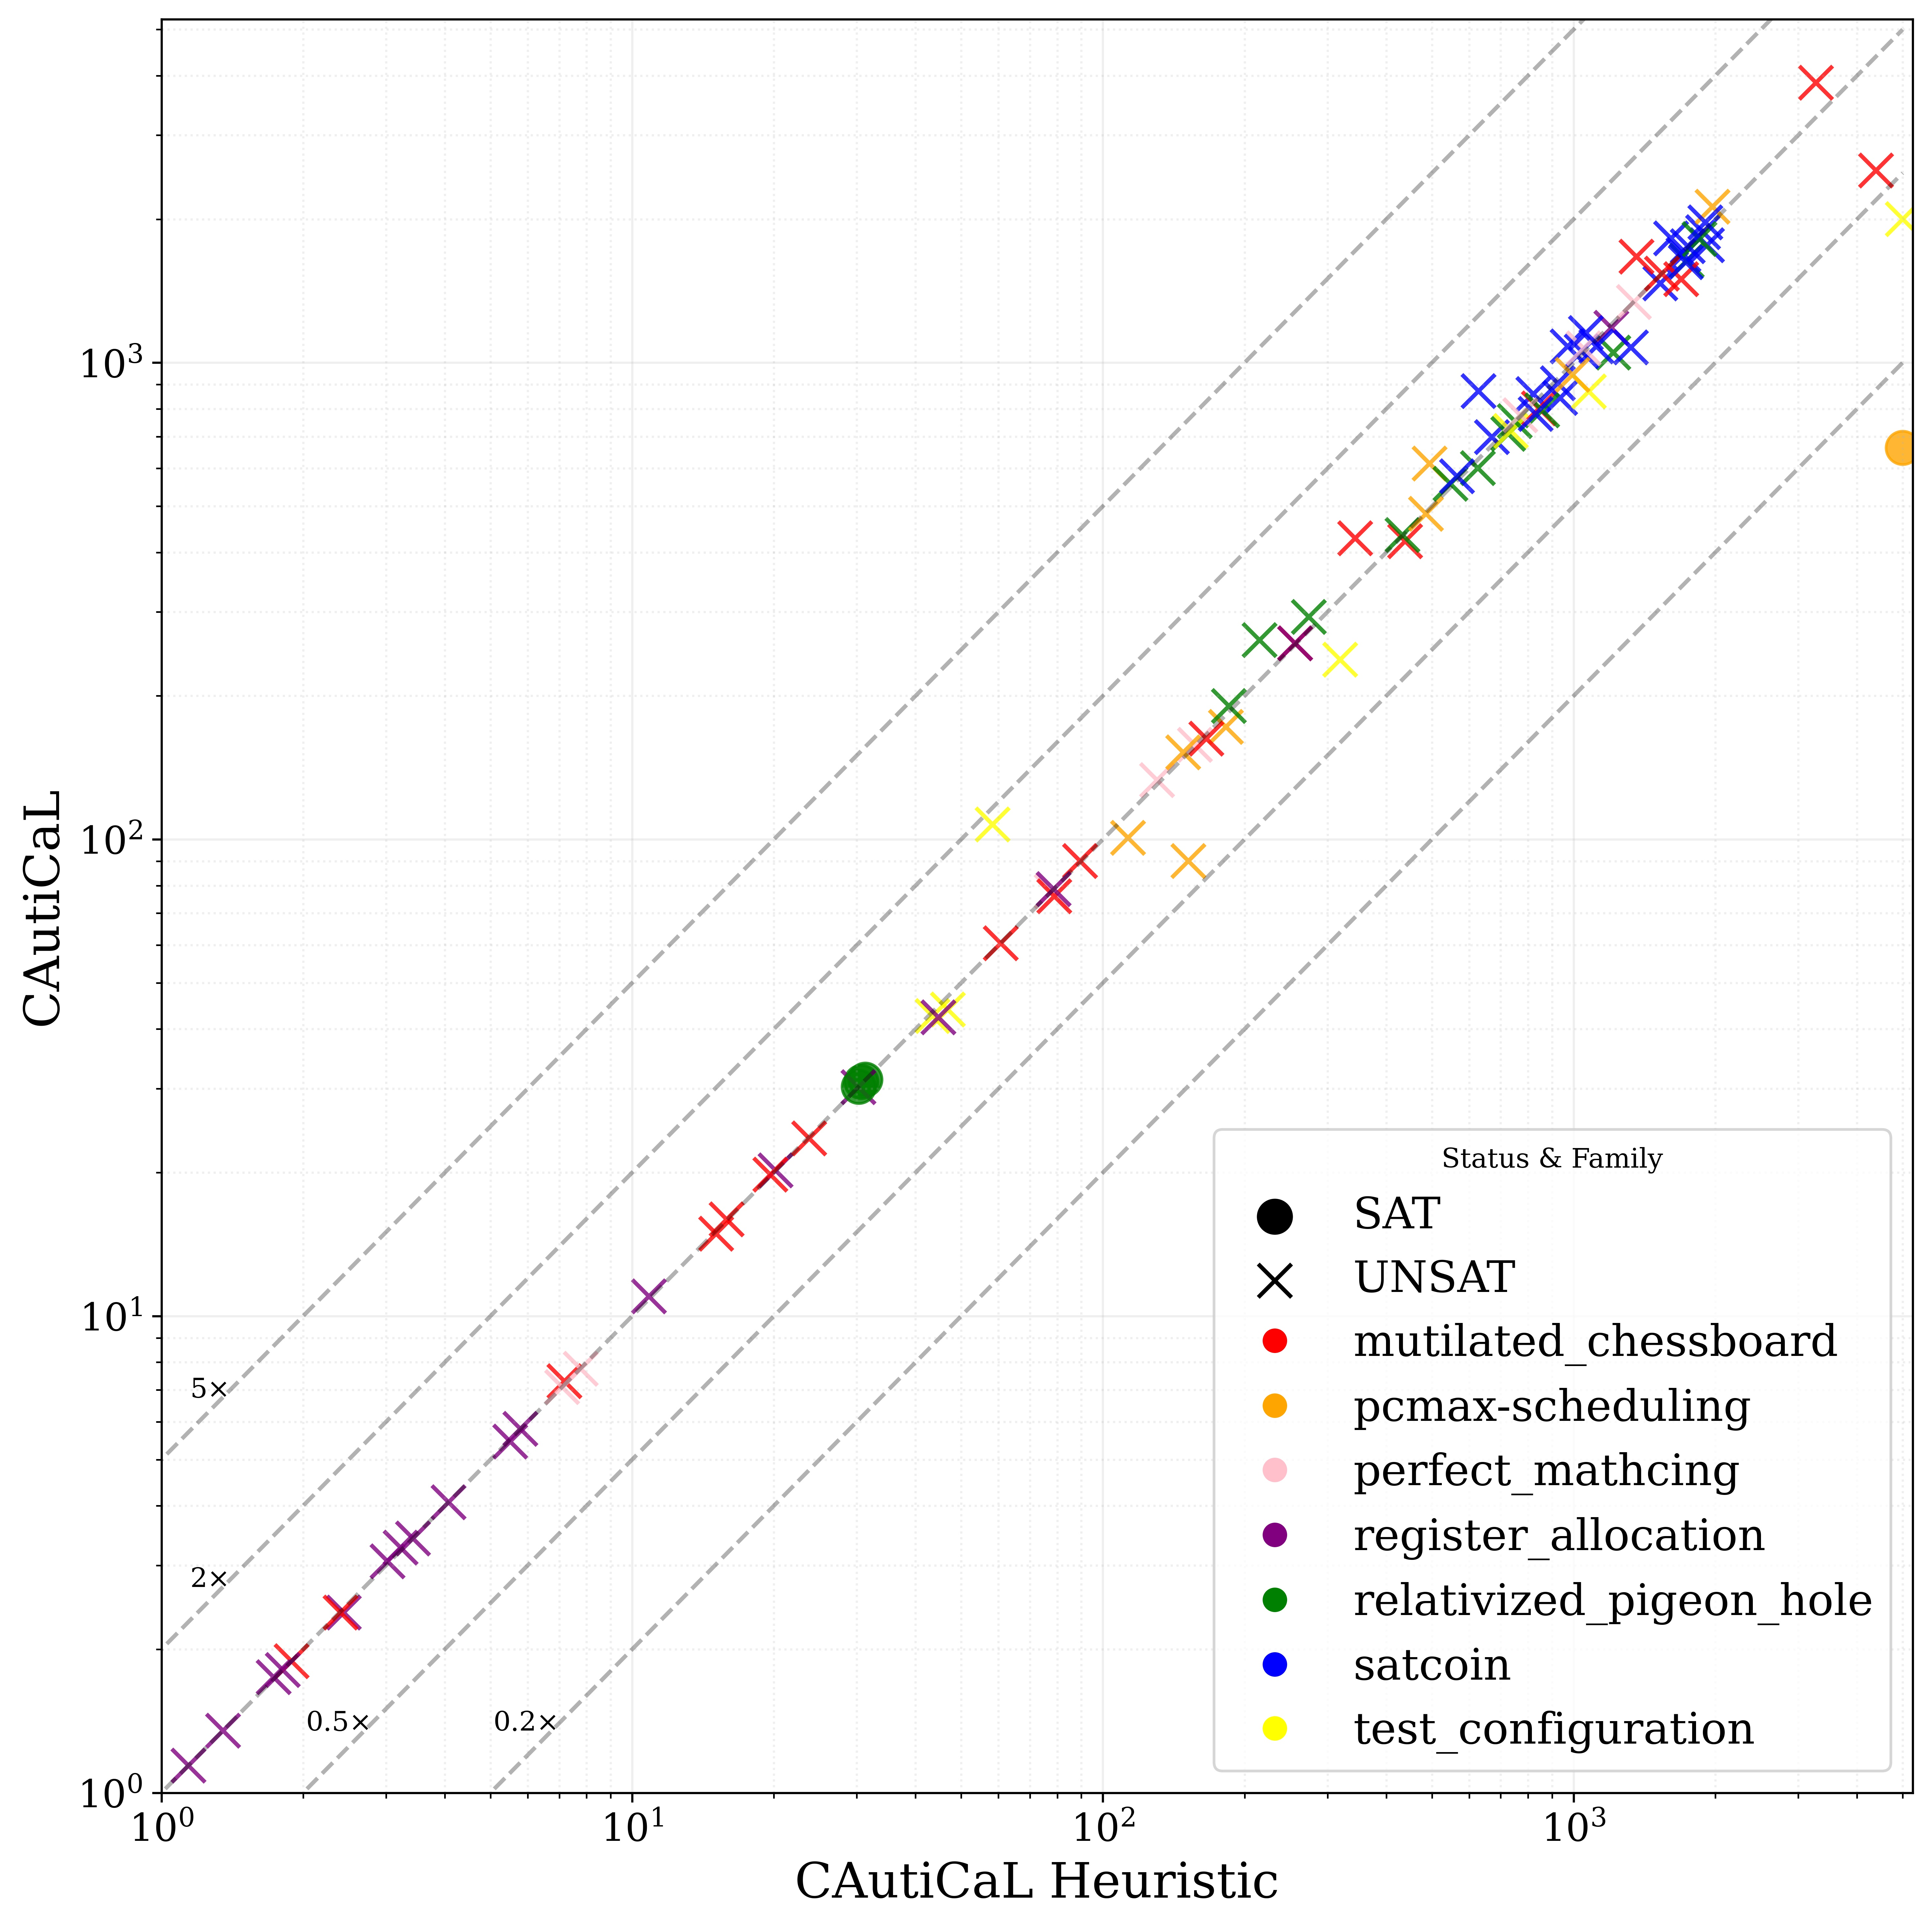
\includegraphics[width=\textwidth]{figs/globaltouch_heuristic_comparison.jpg}
        \caption{Touched heuristic}
        \label{fig:global-touched}
    \end{subfigure}
    \caption{Performance comparison of \tool with other solvers}
\end{figure*}